\section{Practicality of VRF-based mining}
\label{sec:practicality}

In this section, we experimentally show that VRF-based mining is easy to implement and introduces negligible overhead compared to hash-based mining.
First, we show that VRFs can be much more efficient than hash functions used for mining, including Scrypt and CryptoNight.
Second, we profile the performance of $\mathsf{VRFHash}$, and show that the elliptic curve scalar multiplication dominates $\mathsf{VRFHash}$'s runtime, which can be optimised in the future.

\subsection{Experimental setting}

We implement the standardised EC-VRF in Algorithm~\ref{algo:standard-ecvrf} using Go programming language, without any optimisation.
We use Ed25519~\cite{bernstein2012high} as the underlying elliptic curve, Elligator~\cite{bernstein2013elligator} as $H_1(\cdot)$, SHA-3 as the hash function.
Ed25519, SHA-3 and the encoding of points on Ed25519 are supported by Go's standard library.
We use open-source implementations of SHA256D~\footnote{\url{https://github.com/seehuhn/sha256d}}, Scrypt~\footnote{\url{https://github.com/elithrar/simple-scrypt}}, and CryptoNight~\footnote{\url{https://github.com/Equim-chan/cryptonight}}.
All experiments run on a MacBook Pro with a 2.2 GHz Intel Core i7 Processor and a 16 GB DDR4 RAM.
Each group of experiments consists of ten runs, and we take the average value of ten values as the result.

\begin{figure}[htbp]
    \centering
    \begin{subfigure}[]{0.45\textwidth}
        \centering
        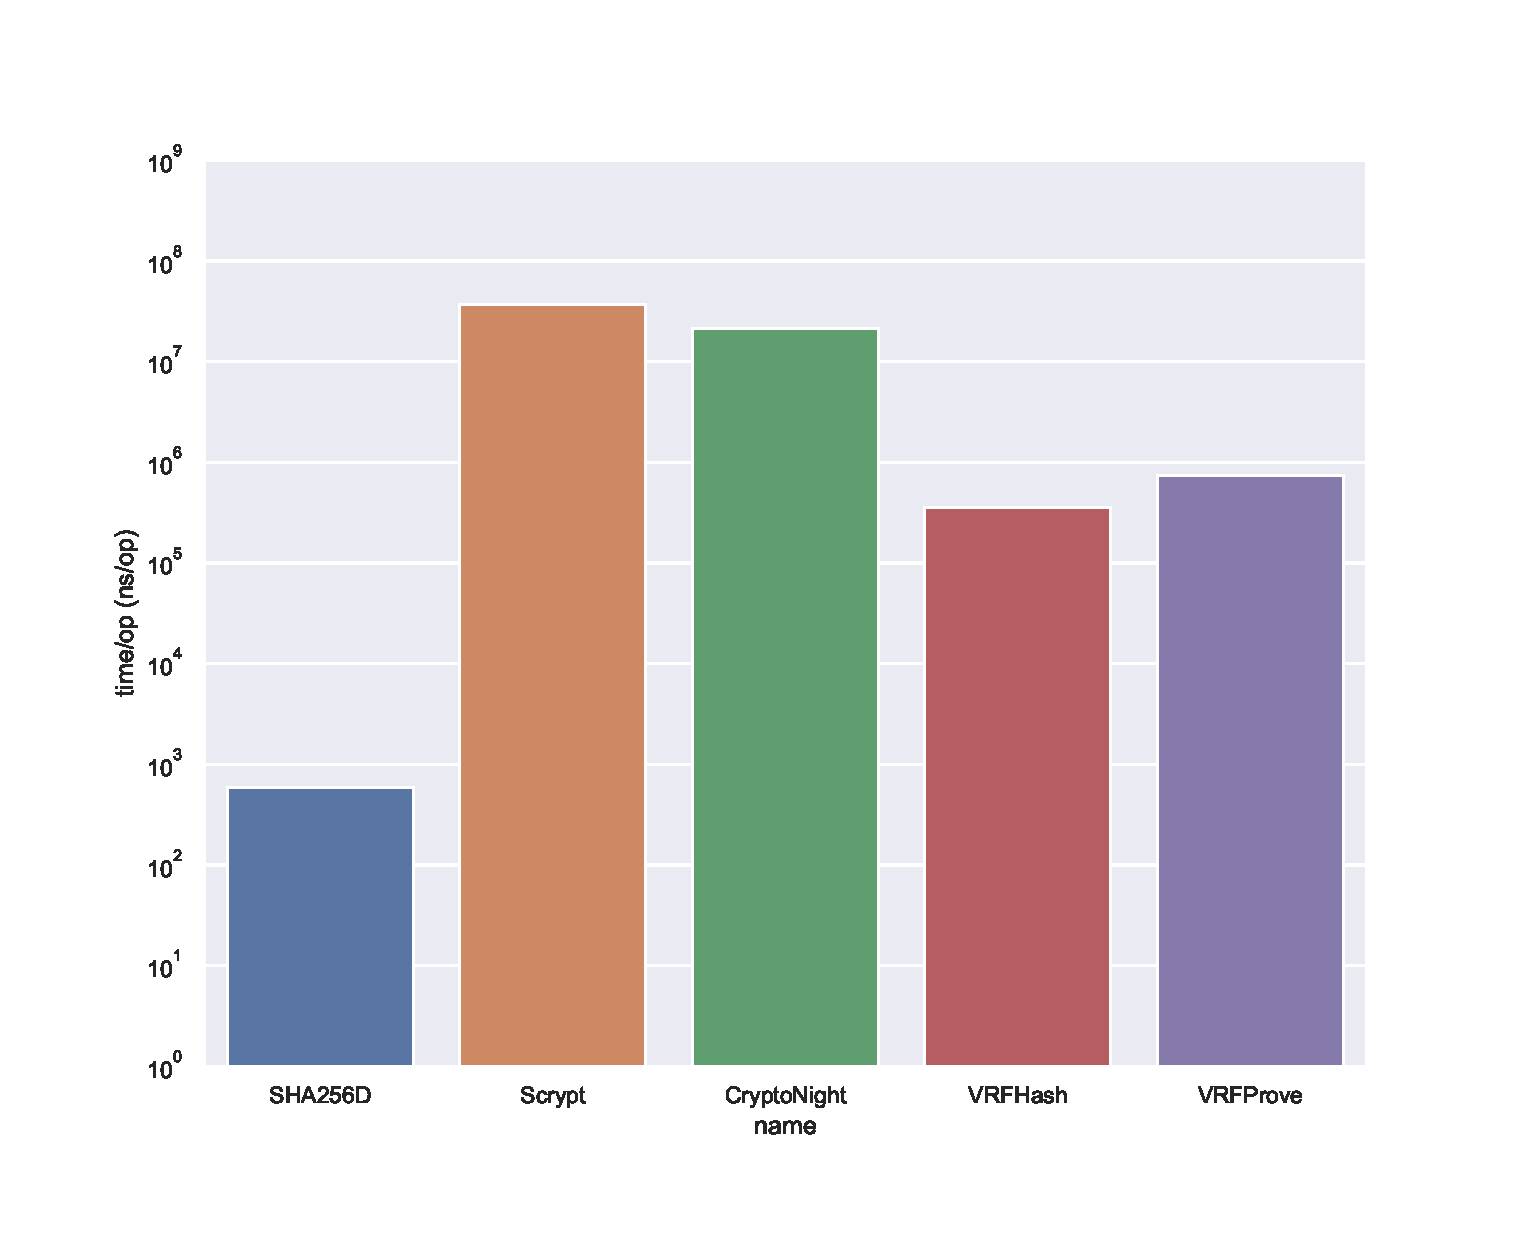
\includegraphics[width=\linewidth]{figs/runtime-comparison.eps}
        \caption{Comparing the runtime of VRF and other mining algorithms.}
        \label{fig:runtime-comparison}
    \end{subfigure}
    \hfill
    \begin{subfigure}[]{0.45\textwidth}
        \centering
        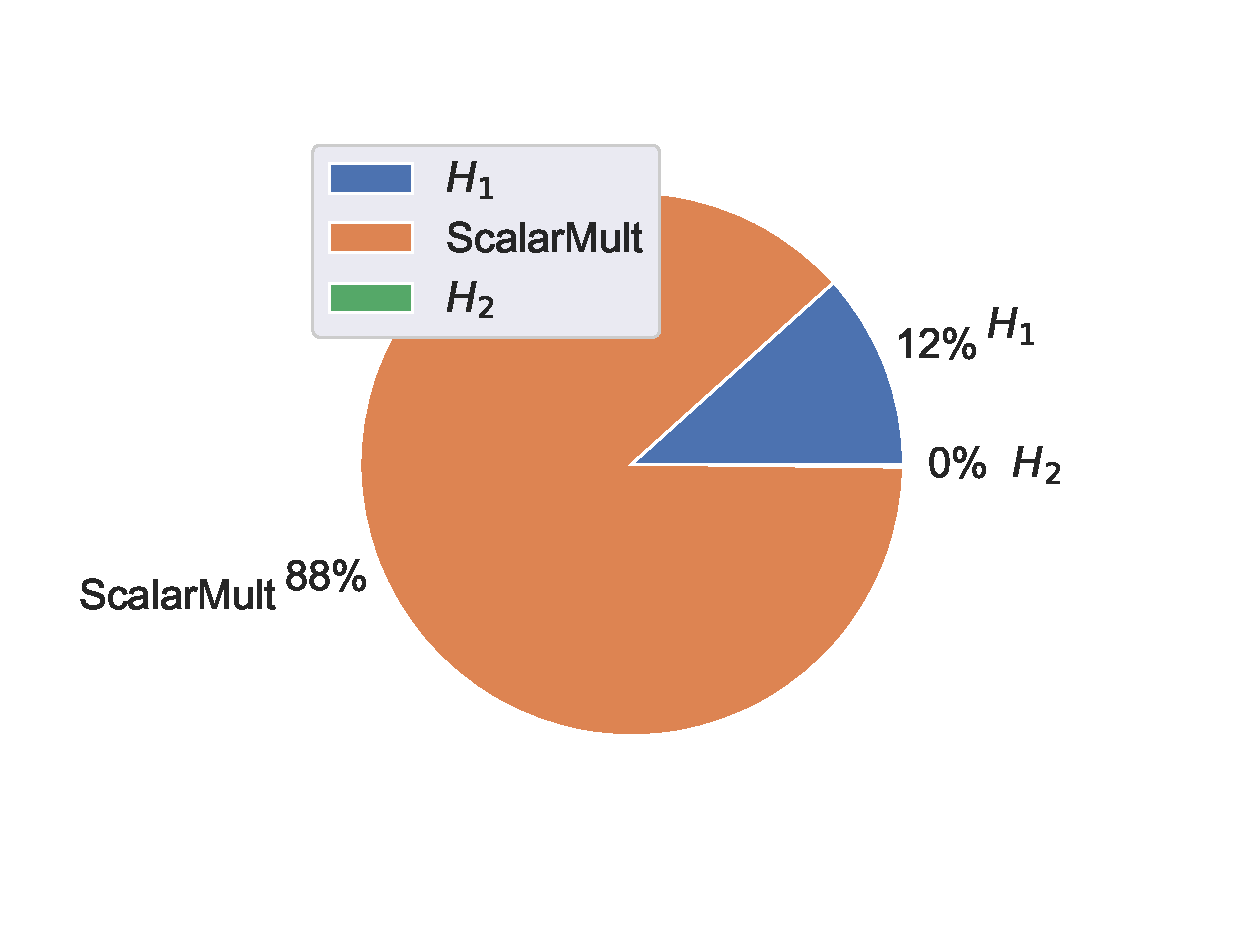
\includegraphics[width=\linewidth]{figs/runtime-breakdown.eps}
        \caption{Runtime breakdown of $\mathsf{VRFHash}$.}
        \label{fig:runtime-breakdown}
    \end{subfigure}
    \caption{Evaluation of VRF.}
\end{figure}

\subsection{VRF v.s. existing mining algorithms}

We compare the performance of VRF with existing mining algorithms.
Figure~\ref{fig:runtime-comparison} shows the runtime of VRF and other algorithms.
SHA256D is much faster than other algorithms, as SHA256D is simply executing SHA256 twice.
In addition, $\mathsf{VRFVerify}$ is slightly slower than $\mathsf{VRFProve}$, and $\mathsf{VRFProve}$ is slightly slower than $\mathsf{VRFHash}$.
Last, although without optimisation, all functions of VRF are much faster than Scrypt and CryptoNight.
This means that VRF is easy to implement and introduces negligible overhead compared to hash functions for mining, so suitable for cryptocurrency mining.



\subsection{Runtime breakdown of VRF}

We profile $\mathsf{VRFHash}$ by evaluating its runtime of each step.
Figure~\ref{fig:runtime-breakdown} shows that, the elliptic curve scalar multiplication $\gamma \gets h^{sk}$ takes 88\% of $\mathsf{VRFHash}$'s running time.
This is because we use SHA-3 as the hash function in $H_1(\cdot)$ and $H_2(\cdot)$, and SHA-3 is designed to be fast.
Meanwhile, we calculate the elliptic curve scalar multiplication using the trivial double-and-add method without any optimisation, thus is much slower than $H_1(\cdot)$ and $H_2(\cdot)$.
Even so, $\mathsf{VRFHash}$ is still much faster than Scrypt and CryptoNight.
This further proves that VRFs introduce negligible overhead compared to hash functions for mining.